
\paragraph{Monkeys exhibit biases} %hallmarks of color category behavior

The animals examined show a hallmark of color categorization behavior: memory biases towards a set of particular points in a perceptually uniform colorspace.
In \autoref{fig:BiasCurves} it can be seen that the biases deviate substantially and systematically from zero, with the attractor points being found where the bias line crosses the zero line from positive to negative (going counter-clockwise). These points are highlighted with colored lines, with the filled areas around these lines showing the confidence intervals on these crossing points. Repeller points found where the line crosses the zero line from negative to positive.

\begin{figure}
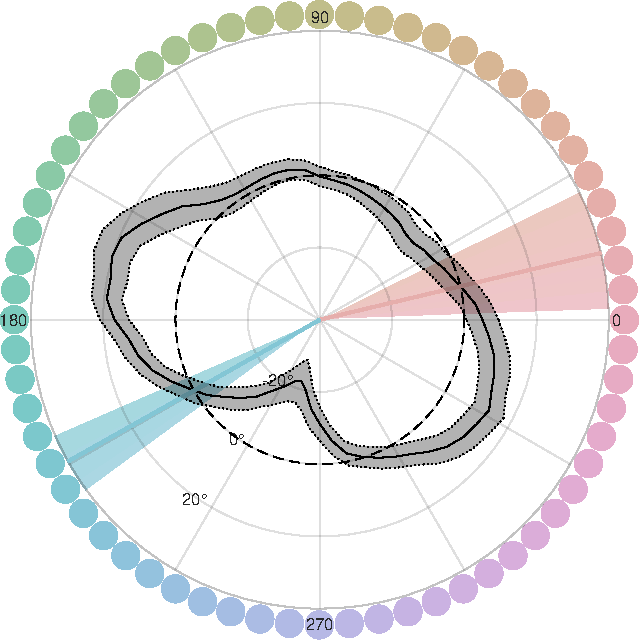
\includegraphics[width=\linewidth]{../../../Analyses/combined/combined_categorybias2_230225.pdf}
\caption{\textbf{Bias as a function of hue, for data collapsed over 4 animals.} 
}
\label{fig:BiasCurvesCombined}
\end{figure}

\paragraph{Shared color categories across monkeys}

We see that all tested monkeys share two common attractor points, which we interpret as evidence of two shared color categories: a warm/orange-ish category (between 0$^\circ$ and 45$^\circ$), and a cool/blue-ish category (between 180$^\circ$ and 225$^\circ$).

\paragraph{Individual differences between monkeys}

In one animal we see evidence of additional categories: strong evidence for a greenish category and weak evidence for a purple category (the ``strength" of a category can be gleaned from looking at the local gradient at the zero-crossing point)

\begin{figure}
    \centering
    \begin{subfigure}[b]{0.49\textwidth}
         \centering
         \caption{}
         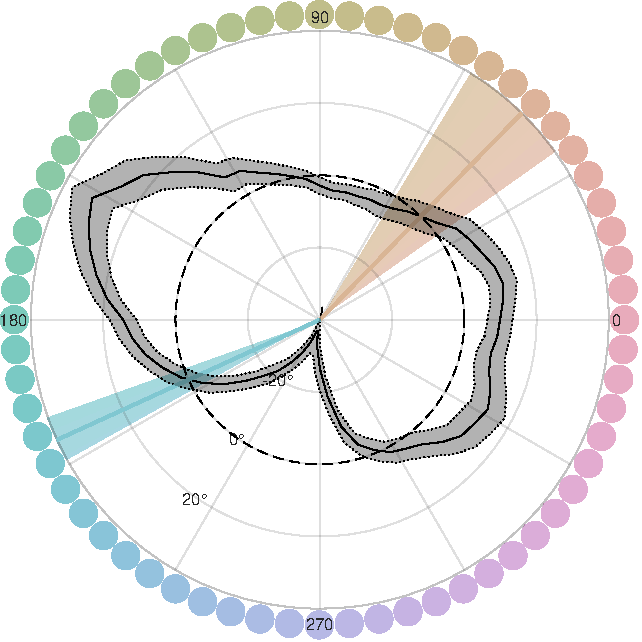
\includegraphics[width=\textwidth]{../../../Analyses/211012_124119_Pollux/210422--211012_Pollux_categorybias2_230225.pdf}
         \label{fig:BiasCurvesPollux}
    \end{subfigure}
    \hfill
    \begin{subfigure}[b]{0.49\textwidth}
         \centering
         \caption{}
         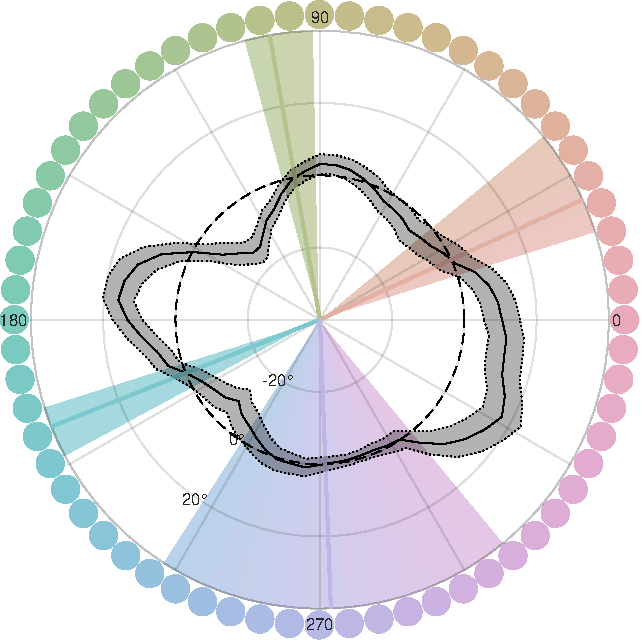
\includegraphics[width=\textwidth]{../../../Analyses/211108_090705_Castor/210517--211108_Castor_categorybias2_230225.pdf}    
         \label{fig:BiasCurvesCastor}
    \end{subfigure}
    
    \begin{subfigure}[b]{0.49\textwidth}
         \centering
         \caption{}
         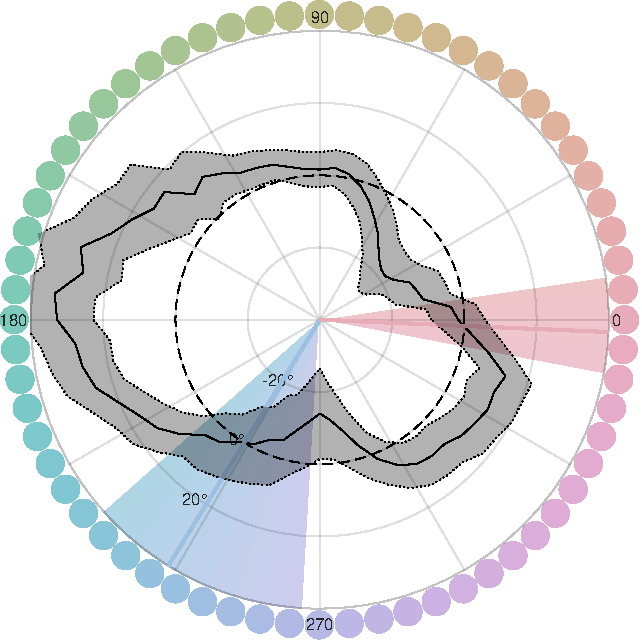
\includegraphics[width=\textwidth]{../../../Analyses/210609_124628_Buster/210428--210609_Buster_categorybias2_230225.pdf}    
         \label{fig:BiasCurvesBuster}
     \end{subfigure}
     \hfill
     \begin{subfigure}[b]{0.49\textwidth}
         \centering
         \caption{}
         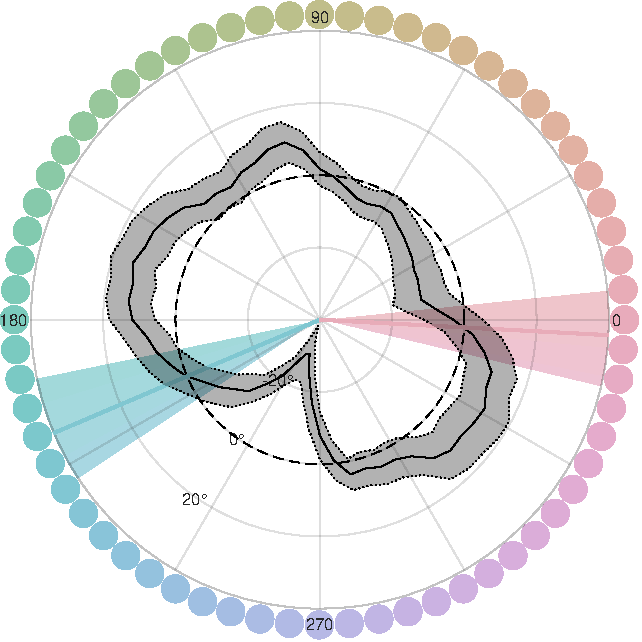
\includegraphics[width=\textwidth]{../../../Analyses/220823_081207_Morty/220322--220823_Morty_categorybias2_230225.pdf}    
         \label{fig:BiasCurvesMorty}
     \end{subfigure}
        \caption{\textbf{Bias curves for individual animals} }
        \label{fig:BiasCurvesIndividual}
\end{figure}

% Results table?

%\begin{figure}
%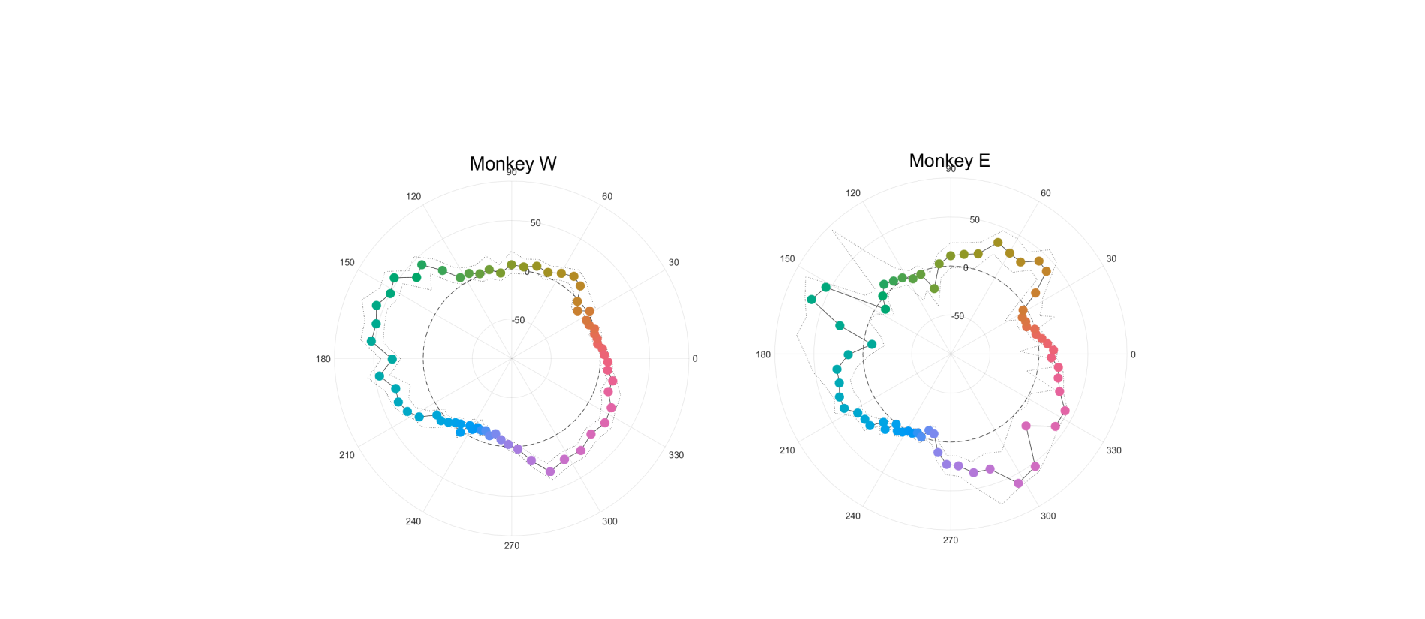
\includegraphics[width=\textwidth]{../../Figures/Old/panichellobias.pdf}
%\caption{Bias as a function of hue, for Panichello monkeys} 
%\end{figure}

\paragraph{Biases Compared to Humans}

Comparison to \cite{bae_why_2015}

Comparison to \cite{panichello_error-correcting_2019}

\paragraph{Cognitive Bias vs. Non-uniformity in Perceptual Space}

\begin{figure}
\includesvg[width=\linewidth]{../../../Analyses/combined/combined_TCC-FreeSimilarityMatrix_230214.svg}
\caption{\textbf{Free Similarity model fit for combined data from all animals}
Similarity between stimulus $s_i$ and stimulus $s_j$, where one is the cue and one is the choice. This is a ``free'' similarity matrix - in that no particular relationship is pre-supposed between any of the stimuli (such as, for example: closer stimuli will be more similar). This figure can be compared to Figure 1D in \cite{schurgin_psychophysical_2020}, except there the rows are circularly shifted so that the the x-axis becomes the relative distance, rather than the absolute value of the stimulus. % should we just plot it the same way at this stage? It doesn't really make a difference here...
% supplementary figure with alternative plotting method?
%confidence intervals?!?!?! !!!!!!!!!!!!!!
} 
\label{fig:SimilarityMatrixCombined}
\end{figure}

\begin{figure}
    \centering
    \begin{subfigure}[b]{0.49\textwidth}
         \centering
         \caption{}
         \includesvg[pretex=\tiny,width=\textwidth]{../../../Analyses/211012_124119_Pollux/210422--211012_Pollux_TCC-FreeSimilarityMatrix_230222.svg}
         \label{fig:SimilarityMatrixPollux}
    \end{subfigure}
    \hfill
    \begin{subfigure}[b]{0.49\textwidth}
         \centering
         \caption{}
         \includesvg[pretex=\tiny,width=\textwidth]{../../../Analyses/211108_090705_Castor/TCC_Castor_20230225.svg}    
         \label{fig:SimilarityMatrixCastor}
    \end{subfigure}
    
    \begin{subfigure}[b]{0.49\textwidth}
         \centering
         \caption{}
         \includesvg[pretex=\tiny,width=\textwidth]{../../../Analyses/210609_124628_Buster/210428--210609_Buster_TCC-FreeSimilarityMatrix230213}    
         \label{fig:SimilarityMatrixBuster}
     \end{subfigure}
     \hfill
     \begin{subfigure}[b]{0.49\textwidth}
         \centering
         \caption{}
         \includesvg[pretex=\tiny,width=\textwidth]{../../../Analyses/220823_081207_Morty/220322--220823_Morty_TCC-FreeSimilarityMatrix_230213.svg}    
         \label{fig:SimilarityMatrixMorty}
     \end{subfigure}
        \caption{\textbf{Free Similarity model fits combined for individual animals} }
        \label{fig:SimilarityMatrixIndividual}
\end{figure}


\paragraph{Longitudinal analysis}

Segmenting our data into subgroups of 5000 datapoints allowed us to both look at whether the determined categories varied over time, and also allowed us to perform a power analysis. From the monkeys studied it was clear that during our data collection period the categories remained static (within our measurement uncertainty), and also that the categories we saw are reliable enough to be seen with substantially less data. See Figures XXX % \autoref{}